
\begin{figure}

\centering

\tikzset{every picture/.style={line width=0.75pt}} %set default line width to 0.75pt        

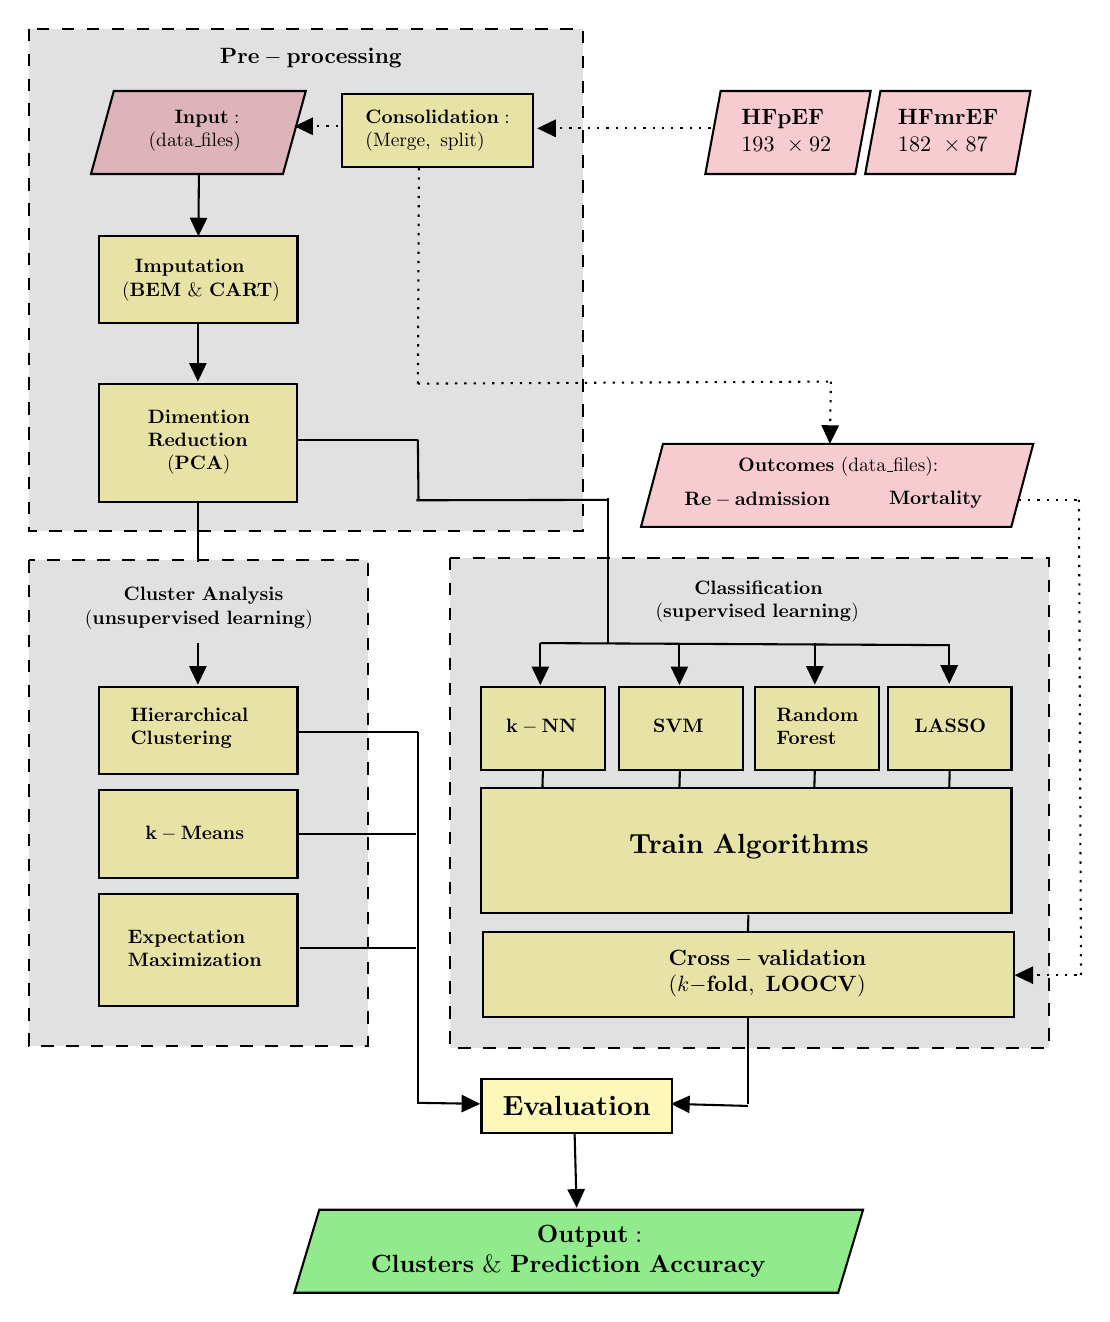
\begin{tikzpicture}[x=0.75pt,y=0.75pt,yscale=-1,xscale=1]
%uncomment if require: \path (0,626); %set diagram left start at 0, and has height of 626

\draw  [fill={rgb, 255:red, 155; green, 155; blue, 155 }  ,fill opacity=0.3 ][dash pattern={on 4.5pt off 4.5pt}]  (2, 5) rectangle (269, 247)   ;
\draw  [fill={rgb, 255:red, 155; green, 155; blue, 155 }  ,fill opacity=0.3 ][dash pattern={on 4.5pt off 4.5pt}]  (205, 260) rectangle (493.5, 496)   ;
\draw  [fill={rgb, 255:red, 155; green, 155; blue, 155 }  ,fill opacity=0.3 ][dash pattern={on 4.5pt off 4.5pt}]  (2, 261) rectangle (165.5, 495)   ;
\draw    (84,75) -- (83.77,103) ;
\draw [shift={(83.75,105)}, rotate = 270.48] [fill={rgb, 255:red, 0; green, 0; blue, 0 }  ][line width=0.75]  [draw opacity=0] (8.93,-4.29) -- (0,0) -- (8.93,4.29) -- cycle    ;

\draw    (83.5,147) -- (83.5,173) ;
\draw [shift={(83.5,175)}, rotate = 270] [fill={rgb, 255:red, 0; green, 0; blue, 0 }  ][line width=0.75]  [draw opacity=0] (8.93,-4.29) -- (0,0) -- (8.93,4.29) -- cycle    ;

\draw    (189.5,344) -- (189.5,523) ;


\draw    (189.5,522.5) -- (217.5,522.97) ;
\draw [shift={(219.5,523)}, rotate = 180.95] [fill={rgb, 255:red, 0; green, 0; blue, 0 }  ][line width=0.75]  [draw opacity=0] (8.93,-4.29) -- (0,0) -- (8.93,4.29) -- cycle    ;

\draw    (248.5,301) -- (248.5,319.22) ;
\draw [shift={(248.5,321.22)}, rotate = 270] [fill={rgb, 255:red, 0; green, 0; blue, 0 }  ][line width=0.75]  [draw opacity=0] (8.93,-4.29) -- (0,0) -- (8.93,4.29) -- cycle    ;

\draw    (315.5,301) -- (315.5,319.22) ;
\draw [shift={(315.5,321.22)}, rotate = 270] [fill={rgb, 255:red, 0; green, 0; blue, 0 }  ][line width=0.75]  [draw opacity=0] (8.93,-4.29) -- (0,0) -- (8.93,4.29) -- cycle    ;

\draw    (380.75,301) -- (380.75,319) ;
\draw [shift={(380.75,321)}, rotate = 270] [fill={rgb, 255:red, 0; green, 0; blue, 0 }  ][line width=0.75]  [draw opacity=0] (8.93,-4.29) -- (0,0) -- (8.93,4.29) -- cycle    ;

\draw    (445.5,301.39) -- (445.5,318.61) ;
\draw [shift={(445.5,320.61)}, rotate = 270] [fill={rgb, 255:red, 0; green, 0; blue, 0 }  ][line width=0.75]  [draw opacity=0] (8.93,-4.29) -- (0,0) -- (8.93,4.29) -- cycle    ;

\draw    (248.5,301) -- (445.5,302) ;


\draw    (348.5,481) -- (348.5,523) ;


\draw    (313.5,523.05) -- (348.5,524) ;

\draw [shift={(311.5,523)}, rotate = 1.55] [fill={rgb, 255:red, 0; green, 0; blue, 0 }  ][line width=0.75]  [draw opacity=0] (8.93,-4.29) -- (0,0) -- (8.93,4.29) -- cycle    ;
\draw  [fill={rgb, 255:red, 248; green, 231; blue, 28 }  ,fill opacity=0.3 ]  (220, 371) rectangle (475.5, 431)   ;
\draw    (281,231) -- (281,301) ;


\draw  [dash pattern={on 0.84pt off 2.51pt}]  (479,232) -- (508,232) ;


\draw  [dash pattern={on 0.84pt off 2.51pt}]  (508,232) -- (509,461) ;


\draw  [dash pattern={on 0.84pt off 2.51pt}]  (479,461) -- (509,461) ;

\draw [shift={(477,461)}, rotate = 0] [fill={rgb, 255:red, 0; green, 0; blue, 0 }  ][line width=0.75]  [draw opacity=0] (8.93,-4.29) -- (0,0) -- (8.93,4.29) -- cycle    ;
\draw  [fill={rgb, 255:red, 248; green, 231; blue, 28 }  ,fill opacity=0.3 ]  (36, 105) rectangle (131.5, 147)   ;
\draw  [fill={rgb, 255:red, 248; green, 231; blue, 28 }  ,fill opacity=0.3 ]  (35.75, 176) rectangle (131.25, 233)   ;
\draw  [fill={rgb, 255:red, 248; green, 231; blue, 28 }  ,fill opacity=0.3 ]  (36, 322) rectangle (131.5, 364)   ;
\draw  [fill={rgb, 255:red, 248; green, 231; blue, 28 }  ,fill opacity=0.3 ]  (36, 372) rectangle (131.5, 414)   ;
\draw  [fill={rgb, 255:red, 248; green, 231; blue, 28 }  ,fill opacity=0.3 ]  (36, 422) rectangle (131.5, 476)   ;
\draw    (131.5,344) -- (189.5,344) ;


\draw    (131.5,393) -- (188.5,393) ;


\draw    (132.5,448) -- (188.5,448) ;


\draw    (188.8,232.2) -- (281,232) ;


\draw    (189.5,203) -- (189.8,232.2) ;


\draw    (131.5,203) -- (189.5,203) ;


\draw  [fill={rgb, 255:red, 248; green, 231; blue, 28 }  ,fill opacity=0.3 ]  (220, 322) rectangle (279.5, 362)   ;
\draw  [fill={rgb, 255:red, 248; green, 231; blue, 28 }  ,fill opacity=0.3 ]  (286.5, 322) rectangle (346, 362)   ;
\draw  [fill={rgb, 255:red, 248; green, 231; blue, 28 }  ,fill opacity=0.3 ]  (352, 322) rectangle (411.5, 362)   ;
\draw  [fill={rgb, 255:red, 248; green, 231; blue, 28 }  ,fill opacity=0.3 ]  (416, 322) rectangle (475.5, 362)   ;
\draw    (249.5,371) -- (249.75,362) ;


\draw    (315.5,371) -- (315.75,362) ;


\draw    (380.5,371) -- (380.75,362) ;


\draw    (445.5,371) -- (445.75,362) ;


\draw  [fill={rgb, 255:red, 248; green, 231; blue, 28 }  ,fill opacity=0.3 ]  (221, 440) rectangle (476.5, 481)   ;
\draw    (83.5,233) -- (83.5,262) ;


\draw    (348.5,440) -- (348.75,432) ;


\draw    (265,537) -- (265.94,571) ;
\draw [shift={(266,573)}, rotate = 268.40999999999997] [fill={rgb, 255:red, 0; green, 0; blue, 0 }  ][line width=0.75]  [draw opacity=0] (8.93,-4.29) -- (0,0) -- (8.93,4.29) -- cycle    ;

\draw  [fill={rgb, 255:red, 208; green, 2; blue, 27 }  ,fill opacity=0.2 ] (335.38,35) -- (407.64,35) -- (400.26,75) -- (328,75) -- cycle ;
\draw    (83.5,301) -- (83.5,319) ;
\draw [shift={(83.5,321)}, rotate = 270] [fill={rgb, 255:red, 0; green, 0; blue, 0 }  ][line width=0.75]  [draw opacity=0] (8.93,-4.29) -- (0,0) -- (8.93,4.29) -- cycle    ;

\draw  [dash pattern={on 0.84pt off 2.51pt}]  (189.5,176) -- (388.5,175) ;


\draw  [dash pattern={on 0.84pt off 2.51pt}]  (388.5,175) -- (388.03,203) ;
\draw [shift={(388,205)}, rotate = 270.95] [fill={rgb, 255:red, 0; green, 0; blue, 0 }  ][line width=0.75]  [draw opacity=0] (8.93,-4.29) -- (0,0) -- (8.93,4.29) -- cycle    ;

\draw  [dash pattern={on 0.84pt off 2.51pt}]  (189.5,176) -- (190,72) ;


\draw  [dash pattern={on 0.84pt off 2.51pt}]  (132,52) -- (152,52) ;

\draw [shift={(130,52)}, rotate = 0] [fill={rgb, 255:red, 0; green, 0; blue, 0 }  ][line width=0.75]  [draw opacity=0] (8.93,-4.29) -- (0,0) -- (8.93,4.29) -- cycle    ;
\draw  [dash pattern={on 0.84pt off 2.51pt}]  (249,53) -- (331,53) ;

\draw [shift={(247,53)}, rotate = 0] [fill={rgb, 255:red, 0; green, 0; blue, 0 }  ][line width=0.75]  [draw opacity=0] (8.93,-4.29) -- (0,0) -- (8.93,4.29) -- cycle    ;
\draw  [fill={rgb, 255:red, 208; green, 2; blue, 27 }  ,fill opacity=0.2 ] (43,35) -- (135.5,35) -- (124.5,75) -- (32,75) -- cycle ;
\draw  [fill={rgb, 255:red, 139; green, 233; blue, 134 }  ,fill opacity=0.95 ] (142,574) -- (404,574) -- (392,614) -- (130,614) -- cycle ;
\draw  [fill={rgb, 255:red, 208; green, 2; blue, 27 }  ,fill opacity=0.2 ] (307.6,205) -- (486,205) -- (475.4,245) -- (297,245) -- cycle ;
\draw  [fill={rgb, 255:red, 208; green, 2; blue, 27 }  ,fill opacity=0.2 ] (412.38,35) -- (484.64,35) -- (477.26,75) -- (405,75) -- cycle ;

\draw (82,54) node [scale=0.7]  {$ \begin{array}{l}
\ \ \ \ \mathbf{Input:}\\
(\mathrm{data\_files})
\end{array}$};
\draw (85,126) node [scale=0.7]  {$ \begin{array}{l}
\ \ \mathbf{Imputation}\\
\mathbf{( BEM\ \&\ CART)}
\end{array}$};
\draw (84,204) node [scale=0.7]  {$ \begin{array}{l}
\mathbf{Dimention}\\
\mathbf{Reduction}\\
\ \ \ \mathbf{( PCA)}
\end{array}$};
\draw (81,342) node [scale=0.7]  {$ \begin{array}{l}
\mathbf{Hierarchical\ }\\
\mathbf{Clustering}
\end{array}$};
\draw (82,393) node [scale=0.7]  {$\mathbf{k-Means}$};
\draw (82,449) node [scale=0.7]  {$ \begin{array}{l}
\mathbf{Expectation}\\
\mathbf{Maximization}
\end{array}$};
\draw (84,284) node [scale=0.7]  {$ \begin{array}{l}
\ \ \ \ \ \ \mathbf{Cluster\ Analysis}\\
\mathbf{( unsupervised\ learning)}
\end{array}$};
\draw  [fill={rgb, 255:red, 248; green, 231; blue, 28 }  ,fill opacity=0.3 ]   (220.16, 511) rectangle (311.84, 537)   ;
\draw (266,524) node   {$\mathbf{Evaluation}$};
\draw (249,341) node [scale=0.7]  {$\mathbf{k-NN}$};
\draw (315,341) node [scale=0.7]  {$\mathbf{SVM}$};
\draw (382,342) node [scale=0.7]  {$ \begin{array}{l}
\mathbf{Random}\\
\mathbf{Forest}
\end{array}$};
\draw (446,341) node [scale=0.7]  {$\mathbf{LASSO}$};
\draw (349,460) node [scale=0.8]  {$ \begin{array}{l}
\ \ \ \ \ \mathbf{Cross-validation}\\
\ \ \ \ \ \mathbf{(} k\mathbf{-fold} ,\ \mathbf{LOOCV)}
\end{array}$};
\draw (353,281) node [scale=0.7]  {$ \begin{array}{l}
\ \ \ \ \ \ \mathbf{Classification}\\
\mathbf{( supervised\ learning)}
\end{array}$};
\draw (349,399) node   {$\mathbf{Train\ Algorithms}$};
\draw (262,594) node [scale=0.9]  {$ \begin{array}{l}
\ \ \ \ \ \ \ \ \ \ \ \ \ \ \ \ \ \ \ \ \mathbf{Output:}\\
\mathbf{Clusters\ \&\ Prediction\ Accuracy}
\end{array}$};
\draw (353,232) node [scale=0.7]  {$\mathbf{Re-admission}$};
\draw (439,232) node [scale=0.7]  {$\mathbf{Mortality}$};
\draw (392,216) node [scale=0.7]  {$\mathbf{Outcomes\ (}\mathrm{data\_files})\mathbf{:}$};
\draw (445,55) node [scale=0.8]  {$ \begin{array}{l}
\mathbf{HFmrEF}\\
182\ \times 87
\end{array}$};
\draw (367,55) node [scale=0.8]  {$ \begin{array}{l}
\mathbf{HFpEF}\\
193\ \times 92
\end{array}$};
\draw  [fill={rgb, 255:red, 248; green, 231; blue, 28 }  ,fill opacity=0.3 ]   (153.05, 36.5) rectangle (244.95, 71.5)   ;
\draw (199,54) node [scale=0.7]  {$ \begin{array}{l}
\mathbf{Consolidation} :\\
(\mathrm{Merge,\ split})
\end{array}$};
\draw (138,19) node [scale=0.8]  {$\mathbf{Pre-processing}$};

\end{tikzpicture}


\caption[Machine learning procedure adopted in the thesis]{\textit{Machine learning procedure adopted in the thesis}}
\label{fig:ML_proc_thesis}
\normalsize
\end{figure}